\documentclass[a4paper]{article}
\usepackage{geometry}
\usepackage{graphicx}
\usepackage{amsmath}
\usepackage{booktabs}
\usepackage{dsfont}
\usepackage{paralist}
\usepackage{epstopdf}
\usepackage{tabularx}
\usepackage{longtable}
\usepackage{multirow}
\usepackage{multicol}
\usepackage[hidelinks]{hyperref}
\usepackage{fancyvrb}
\usepackage{algorithm}
\usepackage{algorithmic}
\usepackage{float}
\usepackage{paralist}
\usepackage[svgname]{xcolor}
\usepackage{enumerate}
\usepackage{array}
\usepackage{times}
\usepackage{url}
\usepackage{fancyhdr}
\usepackage{comment}
\usepackage{environ}
\usepackage{times}
\usepackage{textcomp}
\usepackage{caption}
\usepackage[square,numbers]{natbib}



\urlstyle{rm}



% TO SHOW SOLUTIONS, include following (else comment out):
\newenvironment{soln}{
    \leavevmode\color{blue}\ignorespaces
}{}


\hypersetup{
%    colorlinks,
    linkcolor={red!50!black},
    citecolor={blue!50!black},
    urlcolor={blue!80!black}
}

\geometry{
  top=1in,            % <-- you want to adjust this
  inner=1in,
  outer=1in,
  bottom=1in,
  headheight=3em,       % <-- and this
  headsep=2em,          % <-- and this
  footskip=3em,
}


\title{Gradient Descent for Numerical MAX-CSP} % Title
\author{
Derek Paulsen \\
} 

\date{}

\newcommand{\red}[1]{{\color{red}#1}}
\newcommand{\ind}[1]{\mathds{1}[#1]}
\def \eps{\epsilon}
\begin{document}
\maketitle 


\section{Abstract}
\section{Introduction}

% TODO clean up

Many real world problems can be modeled as constraint 
satisfaction problems. The problems range from logic puzzles 
like sudoku to tuning search engines. Briefly, a constraint satisfaction 
problem is simply the task of finding a valid assignment of variables 
which satisfy as set of constraints. Many classic problems in theoretical computer 
science fit this model, such as the NP-Complete 3-SAT and circuit SAT problems. In this paper 
look variant of CSP, called numerical MAX-CSP. In this variant each variable is a real number
and all of the constraints are linear inequalities, the goal then is to satisfy as 
many linear inequalities as possible. 

The rest of this paper is then structured as follows. First, we give background on the problem 
and the basis for our solution. Next we motivate solving this problem by tying it to 
tuning a keyword search engine with labeled data. We then move on to describe a baseline 
solution by modeling the problem as mixed integer linear program and discuss the issues with 
this solution. Next, we present our algorithm and compare it to the baseline solution. Finally, 
we discuss the experimental results and give directions for future work.

\section{Preliminaries}

In this section we will give an overview of constraint satisfaction problems,
and the specific flavor that we are attempting to tackle in this paper. We then 
give a brief overview gradient descent which is the basis of our proposed solution.

\subsection{Constraint satisfaction problems}

Constraint satisfaction problems (CSPs) encompasses many different problems. Formally a 
constraint satisfaction problem (CSP) is defined as a triple $\langle X, D, C \rangle$ \cite{wiki_CSP}, where 
\begin{align*}
	X &= \{X_1, ..., X_n\} \text{ the set of variables}\\
	D &= \{D_1, ..., D_n\} \text{ the domains of each respective variable}\\
	C &= \{C_1, ..., C_m\} \text{ the set of constraints}\\
\end{align*}
A classic example of a CSP, is the 3-SAT problem. In this case
the boolean variables that appear in at least one clause would be $X$. The domain for 
each variable would be $D_i = \{true, false\}$ and the constraints would all be 
three variable disjunctive clauses. 
In this paper we focus on a subset of CSPs called Numerical MAX-CSP. 
In typical a CSP all constraints must be satisfied, however in MAX-CSP the goal is simply to 
satisfy as may constraints as possible, additionally the domains are the variables 
are numerical (e.g. the real numbers). 

While this problem has certainly been considered before, we were only able to find one previous 
work that directly addresses this issue \cite{num_max_csp_paper}.
In this paper the authors propose a exact solution to numerical MAX-CSP. In particular where 
$D_i = \mathds{R}$ and each constraint $C_j = a_j^Tx \leq b_j, a_j \in \mathds{R}^m, b_j \in \mathds{R}$. 
That is, given a set of linear inequalities, satisfy as many as possible. In the paper the authors 
propose a specific algorithm for this problem based on branch and bound techniques. While the algorithm 
does produce optimal solutions, the algorithm is worst case exponential time.
In fact, this problem is readily to formulated as a mixed integer linear program (MILP),

\begin{align*}
\min_{x,z}\quad &1^Tz\\
s.t. \quad Ax - \epsilon z &\leq b\\
		w &\in \mathds{R}^n\\
		z &\in \{0,1\}^m\\
\end{align*}

Where $\epsilon$ is some large number. The general problem of mixed integer linear programming is 
NP-Hard in general (by reduction to 0-1 integer programming which is NP-Complete \cite{karp_1972}). Hence 
numerical MAX-CSP is likely not to admit an efficient solution. 

\subsection{Gradient Descent}

Gradient descent is an optimization technique which has gained much 
attention in recent years due to the stochastic variant being used in training neural networks for machine learning 
tasks such as computer vision and speech recognition. Despite this focus on machine learning,
gradient descent is a general purpose optimization procedure, capable of optimizing arbitrary 
differentiable functions. Many variations have been proposed in recent years, however
each technique uses the same basic idea. Given a function $f$ and current point $x$, compute $f(x)$. 
Next compute the gradient $\nabla(f(x))$ and update $x$ taking a step in a direction of $-\eta \nabla(f(x))$. Repeat this 
process until the minima of the function is found. 

If $f(x)$ is convex, then gradient descent is guaranteed to find an optimal solution. If $f(x)$ is not convex, 
the gradient descent will converge to a local minimum. Although in the non-convex case, gradient descent 
is not guaranteed, and frequently won't, find the global minimum, it is useful for finding 
minima of functions which are cannot be handled by typical solvers.  This makes it an invaluable tool for 
optimizing functions which don't admit exact optimization techniques such as those used in 
linear programs and quadratic programs.

\section{Motivation}

Numerical MAX-CSPs have a wide variety to applications in such as debugging infeasible 
linear programs, however we are interested in one particular problem, which is that of 
tuning the weights for full search engines. 

Full text search engines are used in a plethora of applications. These search engines (such as Apache Lucene)
are built for efficient retrieval of top-k documents based on a TF/IDF based scoring metric which is dot 
product between two sparse vectors $q^Td = score$\cite{lucene_history} \cite{WAND_paper} \cite{block_max_WAND_paper}.
While this default scoring gives decent results out of the box, 
it is frequently augmented by re-weighting the query $q$, with some weight vector $w$
changing to scoring to be $(q\odot w)^Td = score$. This allows for boosting of certain terms or fields
to improve the quality of search results while not changing the underlying search algorithm. 

The problem we will address in this project is finding a good weight vector $w$. In particular our
problem setting is as follows. We are giving a set of query vectors $Q = \{q_1, ... q_n\}$. For each 
of these query vectors $q_i$ we are given a set of $k$ retrieved document vectors with labels $R_i = \{(d_{i,1}, l_{i,1}), ..., (d_{i, k}, l_{i,k})\}$, 
$l \in \{relevant, irrelevant\}$.
We wish to find a weight vector $w$ that minimizes the number of irrelevant documents that are examined 
before the relevant result is found. This problem can be formulated as a mixed integer linear program (MILP)
as above but with fixed $\gamma < 0$ instead of $b$, in particular,
\begin{align*}
\min_{w,z}\quad &1^Tz\\
s.t. \quad Aw - \epsilon z &\leq \gamma\\
		w &\geq 0\\
		z &\in \{0,1\}\\
\end{align*}

Where each row, $a$, of $A$ comes corresponds to 
$$
a = (d_{i,y} - d_{i,x}) \odot q_i  \quad i \in \{1,...n\} \quad x,y \in \{1,...,k\}, l_{i,x} = relevant, l_{i,y} = irrelevant
$$

That is, the pairwise difference between the components of a matching and non-matching document, multiplied by the 
relevant query. We note that with this setup, 
$$
a^Tw < 0 \implies (q\odot w)^Td_{i,x} > (q\odot w)^Td_{i,y}
$$
That is, the relevant document will be scored higher than the non-relevant document for the query. Solving this 
MILP then corresponds to minimizing the number of irrelevant documents that need to be 
examined in order to find the relevant document for each query. 


\section{Baseline Solutions}

As metioned above we can formulate our problem as a mixed integer linear program 
with binary constraints. In addition, to the mixed integer formulation, we also create an LP
relaxation of the problem as an approximation of the MILP.
The rationale behind this is that the LP relaxation can be solved efficiently and provide a 
deterministic approximation of the MILP. Although the solution could be arbitrarily bad,
we find that the LP typically finds a reasonable solution in much less time 
relative to the MILP. 

\section{Problem with Baseline Solutions}

While modeling the MAX-CSP problem as a MILP is simple solution (at least programming-wise), 
it has a few major issues, namely that depending on the input, the solver time could be exponential in 
the number of constraints. Moreover, even commercial solvers can struggle with large problem sizes, 
either taking large amounts of time to produce any feasible solution or having prohibitive memory requirements.
For our motivating example, we would ideally feed in many labeled queries, 
each producing tens of constraints, hence exponential runtime in the number of constraints greatly 
reduces the usefulness of the solution. 


\section{Our Solution}

To remedy problem of runtime we propose a new solution based on gradient descent. The high level
idea of the solution is simple, begin with a random weight feasible vector $w$ and then perform 
gradient descent until the local minima is found. More specifically we have, 

$$
f(w) = \text{HardTanh}(Aw - \gamma)
$$
Where $ \gamma = -1$ and, 
$$
x\in R, \quad \text{HardTanh}(x) = \begin{cases} -1 \text{ if } x \leq -1\\ 1 \text{ if } x \geq 1\\ x \text{ otherwise}\end{cases}
$$

For gradient updates we start with $\eta = .5$ which decays exponentially every 25 gradient updates. We do a total 
of 500 gradient updates and then back track to find the best $w$ (i.e. the one that satisfies as many constraints as 
possible). We then repeat this process starting with random $w$ until we reach a preset time limit.

\section{Experiments}

We ran our experiments on a server with an AMD Ryzen Threadripper 2950X (16c/32t) processor with 
64GB of RAM. Our MAX-CSP instances are generated from real world datasets, with the number of constraints 
ranging from 7769 to 5994778. For the baseline solutions we 
leverage Gurobi, a commercial solver with an academic license. We choose gurobi because it is consistently 
one of the top performing available solvers \cite{benchmark}.

\begin{tabular}{|l|r|r|r|}
\toprule
Dataset &  \# of Constraints &  \# of Columns &  \% Non-Zero \\
\midrule
         $D_0$ &                   7769 &                 14 &         66.24 \\
         $D_1$ &                  19350 &                 18 &         61.46 \\
         $D_2$ &                 111974 &                 18 &         72.83 \\
         $D_3$ &                 196213 &                 30 &         51.62 \\
         $D_4$ &                3711208 &                124 &         25.09 \\
         $D_5$ &                5994778 &                 22 &         68.58 \\
\bottomrule
\end{tabular}


\begin{figure}
	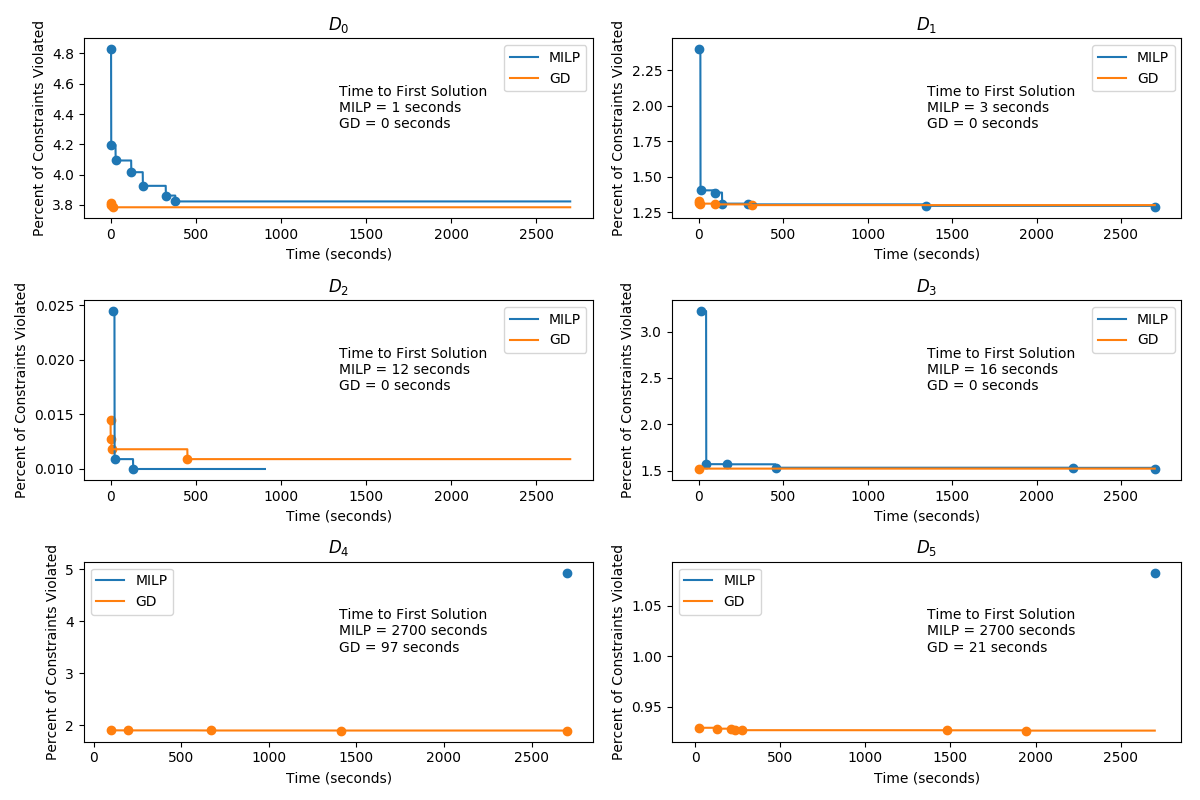
\includegraphics[width=\textwidth]{./time_series.png}
\end{figure}



\section{Discussion}
\section{Future Work}


\bibliographystyle{abbrvnat}
\bibliography{references}
\end{document}
